% Created 2023-02-06 Пн 12:44
% Intended LaTeX compiler: pdflatex
\documentclass[PI, VKR]{HSEUniversity}
         \usepackage{array,tabularx,tabulary,booktabs,longtable,multirow}
         \Year{\the\year{}}
         \supervisor{к.т.н., доцент кафедры информационных технологий в бизнесе НИУ ВШЭ-Пермь}{А. В. Бузмаков}
                  \Abstract{В данной работе проведен анализ этичности разных компаний.

В первой главе находится описание используемых алгоримов.

Во второй главе представлено проектирование системы.

В третьей главе представлена реализация системы.

В четвертой главе представлено тестирование работы системы.

Количество страниц - N, количество иллюстраций - N, количетсво таблиц - N.}


\usepackage[utf8]{inputenc}
\usepackage[T1]{fontenc}
\usepackage{graphicx}
\usepackage{longtable}
\usepackage{wrapfig}
\usepackage{rotating}
\usepackage[normalem]{ulem}
\usepackage{amsmath}
\usepackage{amssymb}
\usepackage{capt-of}
\usepackage{hyperref}
\author{Соломатин Роман Игоревич}
\date{\today}
\title{Разработка сайта для автоматического сбора, анализа и визуализации информации по этичности компаний}
\hypersetup{
 pdfauthor={Соломатин Роман Игоревич},
 pdftitle={Разработка сайта для автоматического сбора, анализа и визуализации информации по этичности компаний},
 pdfkeywords={},
 pdfsubject={},
 pdfcreator={Emacs 28.2 (Org mode 9.6)},
 pdflang={Ru}}
\usepackage{biblatex}
\addbibresource{/home/samoed/Desktop/ESGanalysis/docs/library.bib}
\begin{document}

\maketitle

\chapter*{Введение}
\label{sec:org5986b54}
Этичность компаний уже давно вызывает озабоченность, особенно их поведение в спорных ситуациях и предоставление услуг, ориентированных на клиента. В последние годы все большее внимание уделяется оценке этичности компаний\autocite{mure_esg_2021}, особенно в банковском секторе и через призму экологических, социальных и управленческих факторов (ESG). Необходимость в таких оценках становится все более острой по мере того, как общество продолжает бороться с последствиями неправомерных действий корпораций и более широким воздействием корпоративной деятельности на общество и окружающую среду.

В настоящее время существует несколько сервисов\footnote{test}, которые призваны оценивать этику компании, но эти оценки часто основаны на судебных делах и других официальных отчетах, а не на отзывах клиентов. Это привело к ситуации, когда отдельные лица должны проводить свои собственные исследования, чтобы определить насколько этична компания. Это часто включает в себя просмотр отзывов с различных веб-сайтов, что может занять много времени и не всегда может дать исчерпывающую или точную картину.
Для решения этой проблемы будет реализована система, которая собирала бы и анализировала отзывы потребителей с различных веб-сайтов, чтобы дать более полную и точную оценку этической практики компании. Такая система может быть разработана для автоматического сбора и анализа отзывов потребителей из различных источников, включая социальные сети и сайты отзывов. Затем собранные данные могут быть проанализированы с помощью различных методов, таких как обработка естественного языка и машинное обучение, для выявления закономерностей и тенденций, связанных с этической практикой компании. Полученный анализ может быть использован для разработки более надежной и достоверной системы оценки этичности компаний.
Объект исследования – деятельность компаний.

Предмет исследования – программные средства для оценки этичности деятельности компаний.

Цель работы – создание системы для оценки этичности компаний.

Исходя из поставленной цели, необходимо:

\begin{enumerate}
\item Провести анализ предметной области
\item Провести анализ системы
\item Реализовать систему
\item Провести тестирование системы
\end{enumerate}

Этап анализа должен:
\begin{enumerate}
\item Анализ предметной области
\item Анализ существующих алгоритмов
\end{enumerate}

Этап проектирования должен включать:
\begin{enumerate}
\item Проектирование серверной части
\item Проектирование модели для определения этичности
\item Проектирование клиентской части приложения
\end{enumerate}

Этап реализации должен включать:
\begin{enumerate}
\item Описание сбора данных
\item Реализации модели
\item Реализации серверной части
\item Реализации клиентской части
\end{enumerate}

Этап тестирования должен включать:
\begin{enumerate}
\item Тестирование модели
\item Тестирование серверной части
\item Тестирование клиентской части
\end{enumerate}
\chapter{Анализ предметной области}
\label{sec:orgab43770}
бла бла бла
\section{Способы оценки этичности компаний}
\label{sec:org386b1b1}
Компаниям важно оставаться этичными, так как на долгосрочной перспективе это приносит большую прибыль и улучшает показатели бизнеса, чем неэтичный способ ведение бизнеса\autocites{climent_ethical_2018}[][]{mure_esg_2021}. Насколько этична компания можно рассматривать с двух сторон, самой компании и их клиентов. Со стороны компаний можно выделить факторы, которые можно получить из их отчетности:
\begin{itemize}
\item количество капитала, чтобы они не могли обанкротиться;
\item какое влияние они вносят на окружающую среду;
\item куда идут инвестиции\autocite{harvey1995ethical}.
\end{itemize}
Для пользователей одними из ключевых факторов можно выделить:
\begin{itemize}
\item качество пользовательского сервиса\autocite{brunk2010exploring};
\item насколько навязчивые услуги компании\autocite{mitchell1992bank}.
\end{itemize}

Кроме того, важно отметить, что оценка этики компании -- это не одноразовый процесс, а скорее непрерывная попытка понять и оценить действия, политику и практику компании с течением времени. Это включает в себя рассмотрение соблюдения компанией отраслевых этических стандартов и передовой практики, а также мониторинг любых изменений в этической позиции компании с течением времени. Кроме того, участие в диалоге с компанией и консультации с организациями, специализирующимися на оценке корпоративной ответственности могут дать ценную информацию об этических практиках компании.

В этой работе для анализа текстов будут использоваться алгоритмы машинного обучения.
\section{Анализ существующих решений}
\label{sec:org9e7e1c5}
Сейчас данные об этичности компаний можно получить из агрегаторов отзывов и отчётности компаний. Агрегаторы отзывов позволяют собрать информацию о клиентском обслуживании, а отчетность компаний о положении дел в целом. Но сейчас не существует способов, как можно оценить все вместе.
\section{Алгоритмы для анализа текста}
\label{sec:org3f596cb}
Алгоритмы машинного обучения для анализа текста получили широкое распространение для извлечения информации из неструктурированных данных с помощью больших помеченных наборов данных. Среди различных используемых методов несколько алгоритмов оказались особенно эффективными в этой области. К ним относятся мешок слов\autocite{doi:10.1080/00437956.1954.11659520}, TF-IDF\autocite{jones1972statistical}, Word2Vec\autocite{mikolov2013distributed}, ELMO\autocite{elmo}, GPT\autocite{radford2019language} и BERT\autocite{devlin2018bert}. Каждый из этих алгоритмов обладает уникальными характеристиками, которые делают их хорошо подходящими для определенных приложений.

Модель \label{Мешок слов} представляет текстовые данные путем присвоения уникального номера каждому слову в документе. Этот метод прост в реализации, но не учитывает порядок слов в предложении. С другой стороны, модель TF-IDF представляет текстовые данные, учитывая как частоту слова в документе (TF), так и его редкость во всех документах корпуса (IDF). Этот подход может быть использован для определения важности слова в данном документе и обычно используется в задачах поиска информации и обработки естественного языка, но он не понимает контекста слов.

Word2Vec использует векторное представление слов, что позволяет алгоритму улавливать значение слов в сходных контекстах. Это позволяет более точно и изощренно представлять взаимосвязи между словами, что приводит к повышению производительности в таких задачах, как классификация текста и анализ настроений.

ELMO, GPT и BERT, с другой стороны, основаны на архитектуре трансформеров, в которой каждое предложение представлено вектором чисел, обычно известным как вложение. Такое представление позволяет получить более полное и целостное понимание текста, поскольку оно учитывает контекст всего предложения или текста.

Из этих алгоритмов BERT считается наиболее продвинутым и мощным, поскольку он способен учитывать контекст всего предложения или текста, в то время как GPT и ELMO рассматривают только односторонний контекст. Это позволяет BERT достигать самых современных результатов в широком спектре задач анализа естественного языка.

Также для объединения эмбеддинговых пространств из разных сфер будет работать алгоритм подобный CLIP\autocite{radford2021learning}, только для трансформации текста в текст.
\subsection{BERT}
\label{sec:org05d2de9}
BERT \autocite{devlin2018bert} (Bidirectional Encoder Representations from Transformers) -- это нейросетевая языковая модель, которая относится к классу трансформеров. Она состоит из 12 «базовых блоков» (слоев), а на каждом слое 768 параметров.

На вход модели подается предложение или пара предложений. Затем разделяется на отдельные слова (токены). Потом в начало последовательности токенов вставляется специальный токен \texttt{[CLS]}, обозначающий начало предложения или начало последовательности предложений. Пары предложений группируются в одну последовательность и разделяются с помощью специального токена \texttt{[SEP]}, затем к каждому токену добавляется эмбеддинг, показывающий к какому предложению относится токен. Потом все токены превращаются в эмбеддинги \ref{fig:inputemebeddings} по механизму описаному в работе \autocite{NIPS2017_3f5ee243}.

\begin{figure}[h]
\centering
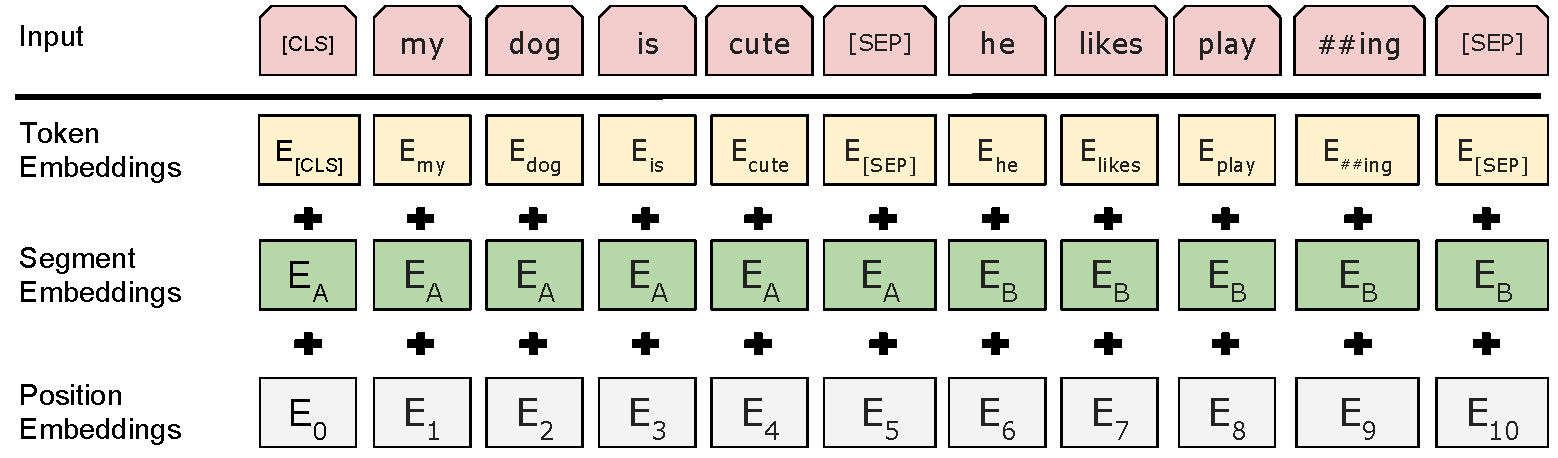
\includegraphics[width=.9\linewidth]{img/Input_Emebeddings.pdf}
\caption{\label{fig:inputemebeddings}Пример ввода текста в модель}
\end{figure}

При обучении модель выполняет на 2 задания:
\begin{enumerate}
\item Предсказание слова в предложении

Поскольку стандартные языковые модели либо смотрят текст слева направо или справа налево \ref{fig:BERT_comparisons}, как ELMo\autocite{elmo} и GPT\autocite{radford2019language}, они не подходят под некоторые типы заданий. Так как BERT двунаправленный, у каждого слова можно посмотреть его контекст, что позволит предсказать замаскированное слово.

\begin{figure}[h]
\centering
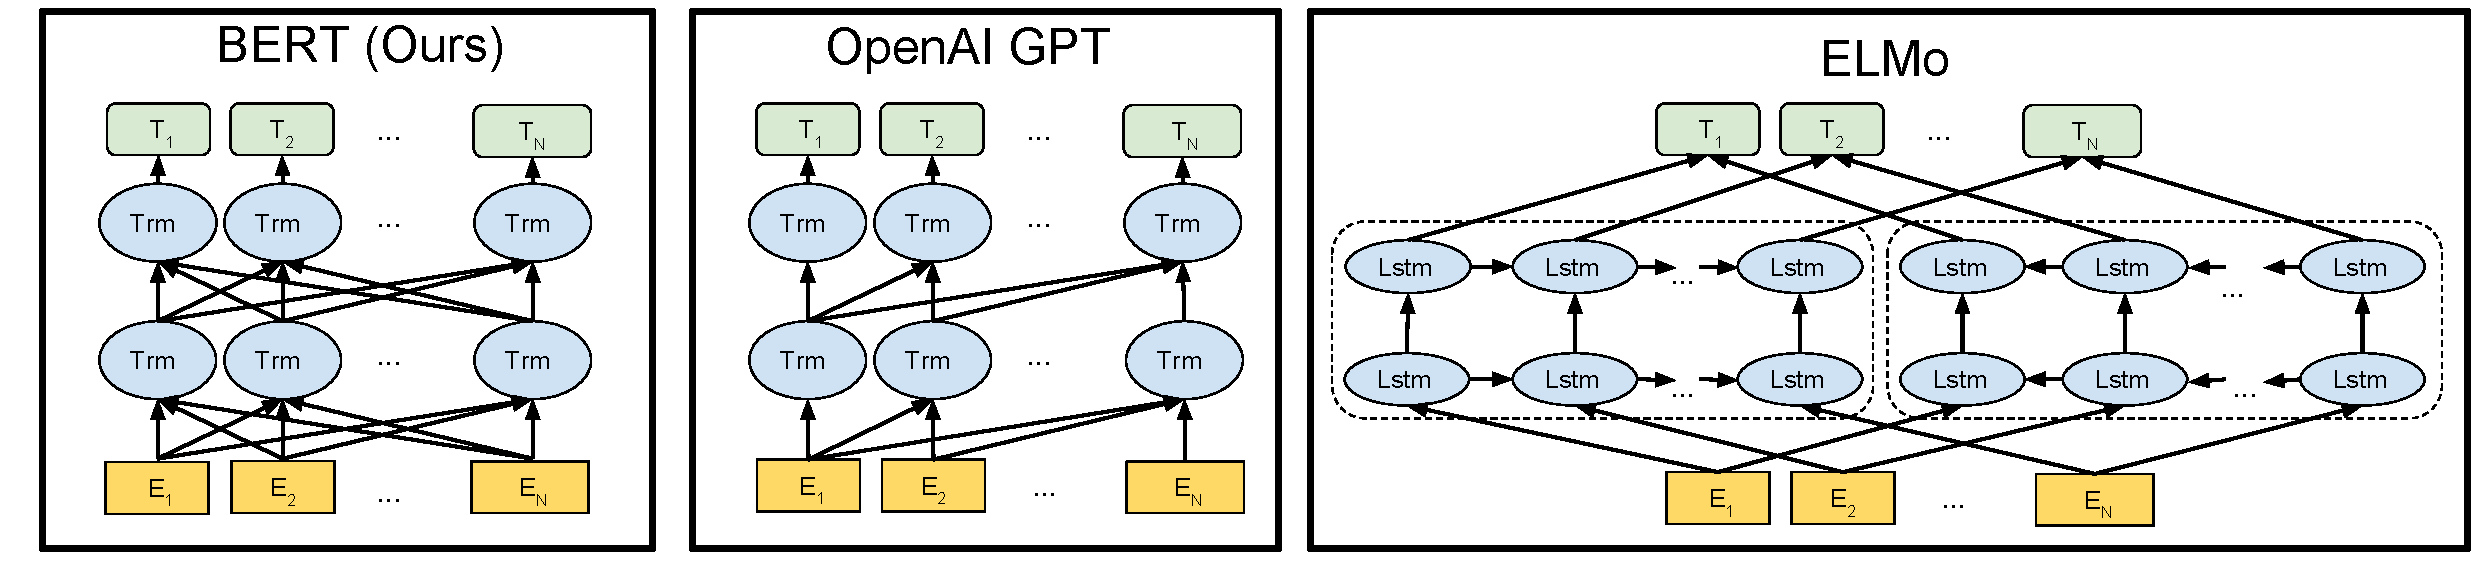
\includegraphics[width=.9\linewidth]{img/BERT_comparisons.pdf}
\caption{\label{fig:BERT_comparisons}Сравнение принципов работы BERT, ELMo, GPT}
\end{figure}

Это задание обучается следующим образом -- 15\% случайных слов заменяются в каждом предложении на специальный токен \texttt{[MASK]}, а затем предсказываются на основании контекста. Однако иногда слова заменяются не на специальны токена, в 10\% заменяются на случайный токен и еще в 10\% заменяются на случайное слово.

\item Предсказание следующего предложения

Для того чтобы обучить модель, которая понимает отношения предложений, она предсказывает, идут ли предложения друг за другом. Для этого с 50\% вероятностью выбирают предложения, которые находятся рядом и наоборот. Пример ввода пары предложений в модель \ref{fig:bert_pretrainin}.

\begin{figure}[hbp]
\centering
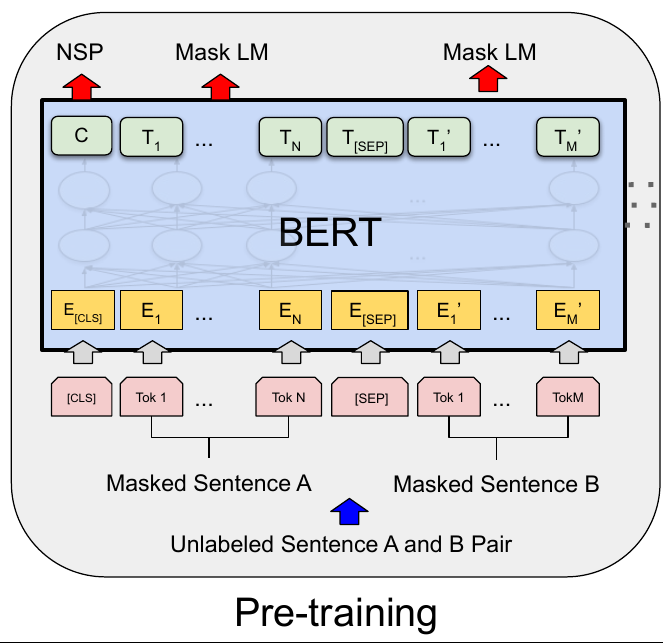
\includegraphics[width=0.6\textwidth]{img/bert_pretrainin.png}
\caption{\label{fig:bert_pretrainin}Схемам работы BERT}
\end{figure}
\end{enumerate}
\subsection{Sentence BERT}
\label{sec:org86b26c2}
Sentense BERT \autocite{reimers-2019-sentence-bert} -- это модификация предобученных моделей BERT, которая использует 2 модели BERT, затем усреднят их выходы, а после с помощью функции ошибки выдаёт результат. Схема работы модели \ref{fig:sbert}.
\begin{figure}[hbp]
\centering
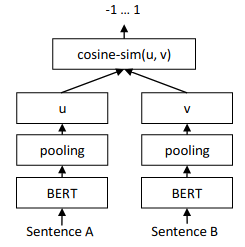
\includegraphics[width=0.6\textwidth]{img/sbert.png}
\caption{\label{fig:sbert}Схема работы SBERT}
\end{figure}
Основное преимущество данной модели над классическим BERT: эмбеддинги предложений можно сравнивать друг с другом независимо и не пересчитывать их пару каждый раз. Например, если для поиска похожих предложений из 10000 для обычного BERT потребуется 50 миллионов вычислений различных пар предложений, и это займёт 50 часов, то Sentense BERT рассчитает эмбеддинг каждого предложения отдельно, потом их сравнит. Такой способ рассчета ускоряет работу программы до 5 секунд.
\subsection{CLIP}
\label{sec:orgc029ed1}
CLIP (Contrastive Language–Image Pre-training)\autocite{radford2021learning} -- это нейронная сеть, обученная на множестве пар (изображение, текст). Его можно проинструктировать на естественном языке, чтобы он предсказал наиболее релевантный фрагмент текста, учитывая изображение, без прямой оптимизации для задачи. Эта модель состоит из двух разных моделей. Одна для кодирования текста в эмбеддинг -- трансформер \autocite{NIPS2017_3f5ee243}, а для кодирования изображения используется vision transformer \autocite{dosovitskiy2020image}. В данной работе будет использована модификация этого метода для сопоставления текстов из разных сфер между собой.

Метод обучения данной модели авторы отнесли к "natural language supervision" (обучение естественным языком). На каждой итерации обучения берется набор пар изображение-текст. Затем они трансформируются в эмбеддинги и к каждому тексту модель пытается подобрать текст, и наоборот. Данный способ позволяет соединить пространства двух различных источников информации.
\chapter{Проектирование системы}
\label{sec:orgee3d8ba}
\section{Проектирование базы данных}
\label{sec:org723332b}

\section{Проектирование архитектуры системы}
\label{sec:org5f3e812}
\subsection{Проектирование серверной части}
\label{sec:org7d29938}
\subsection{Проектирование клиентской части}
\label{sec:org15da838}

\chapter{Реализация системы}
\label{sec:orgeeb2462}
\section{Реализация серверной части}
\label{sec:org7c9c272}
\subsection{Реализация API}
\label{sec:org99853e4}
\subsection{Реализация парсера banki.ru}
\label{sec:org13fe4cd}
\subsection{Реализация парсера sravni.ru}
\label{sec:orgbafd3ea}
\subsection{Реализация модуля обработки текста}
\label{sec:org87076be}
\subsection{Дообучение модели}
\label{sec:org4e15a37}
\section{Реализация клиентской части}
\label{sec:org4892f8a}
\chapter{Тестирование системы}
\label{sec:org48418f6}
\chapter*{Заключение}
\label{sec:orgfebf709}
%\nocite{*}
\putbibliography
\appendix
\end{document}
